\documentclass[svgnames,dvipsnames,hyperref={bookmarks=false},usepdftitle=false]{beamer}
\usetheme{scaladays}
\usepackage{tikz}
\usetikzlibrary[arrows.meta]

\title{State of the Meta, Spring 2015}
\author{Eugene Burmako (\href{https://twitter.com/xeno_by}{@xeno{\textunderscore}by})}
\institute{\'Ecole Polytechnique F\'ed\'erale de Lausanne \\ \texttt{\href{http://scalameta.org/}{http://scalameta.org/}}}
\date{17 March 2015}
\hypersetup{pdfauthor={Eugene Burmako},pdftitle={State of the Meta, Spring 2015}}

\begin{document}

\titleframe

\begin{frame}{scala.meta}
\begin{quote}
The goal of scala.meta is to make metaprogramming easy\only<2->{, ensuring that it:\\}
\only<2->{1) Doesn't require knowledge of compiler internals\\}
\only<3->{2) Is safe from compiler crashes by construction\\}
\only<4->{3) Is portable across a wide range of implementors\\}
\end{quote}
\begin{flushright}
\textemdash\text{ }scalameta.org
\end{flushright}
\end{frame}

\begin{frame}[c, fragile]{ScalaDays Berlin}
\begin{center}
% http://www.utopiaplanitia.info/blueprints.html

\includegraphics[height=7.5cm]{nx-blueprint.jpg}
\end{center}
\end{frame}

\begin{frame}[c, fragile]{ScalaDays San Francisco}
\begin{center}
% http://en.memory-alpha.org/wiki/Phoenix

\includegraphics[height=5cm]{nx-alpha.jpg}
\end{center}
\end{frame}

\begin{frame}{Outline}
\begin{itemize}
\item The next-generation metaprogramming ecosystem
\item Quick introduction into scala.meta
\item Key concepts of the syntactic API
\item Key concepts of the semantic API
\end{itemize}
\end{frame}

\begin{frame}{Credits}
Big thanks to everyone who helped turning scala.meta into reality!

\begin{tabular}{p{0.4\textwidth}p{0.5\textwidth}}
\begin{itemize}
\itemsep0.5em
\item Uladzimir Abramchuk
\item Eric Beguet
\item Igor Bogomolov
\item Eugene Burmako
\item Mathieu Demarne
\item Martin Duhem
\item Adrien Ghosn
\item Vojin Jovanovic
\item Guillaume Mass\'e
\end{itemize} &
\begin{itemize}
\itemsep0.5em
\item Mikhail Mutcianko
\item Dmitry Naydanov
\item Artem Nikiforov
\item Vladimir Nikolaev
\item Martin Odersky
\item Alexander Podkhalyuzin
\item Jatin Puri
\item Dmitry Petrashko
\item Denys Shabalin
\end{itemize} \\
\end{tabular}
\end{frame}

\sectionframe{Part 1: The next-generation metaprogramming ecosystem}

\begin{frame}{High-level view}
\begin{itemize}
\item scala.reflect has known issues, but it works and is well-understood
\item What does scala.meta have to offer, concretely?
\item Here's our proposed design of the future metaprogramming ecosystem
\item There's work being done towards implementing it as we speak
\end{itemize}
\end{frame}

\begin{frame}[fragile]{Architecture in a nutshell}
\begin{itemize}
\item<3-> Ecosystem of platform-independent metaprograms\\
macros, style checkers, code formatters, refactorings,\\
... (other tools, utilities, libraries)
\vskip20pt
\item<1-> Library of platform-independent metaprogramming APIs\\
\texttt{\href{https://github.com/scalameta/scalameta}{https://github.com/scalameta/scalameta}}
\vskip20pt
\item<2-> Collection of platform-dependent implementations\\
\texttt{\href{https://github.com/scalameta/scalahost}{https://github.com/scalameta/scalahost}},\\
... (intellij, dotty, etc)
\end{itemize}
\end{frame}

\begin{frame}[fragile]
\frametitle<1>{Architecture in more detail}
\frametitle<2>{The frontend/backend separation}
\frametitle<3>{Notable frontend metaprograms}
\frametitle<4>{How do metaprograms read TASTY? (Design \#1)}
\frametitle<5>{How do metaprograms read TASTY? (Design \#2)}
\frametitle<6>{What about Dotty?}
\frametitle<7>{Revisiting tools (Design \#1)}
\frametitle<8>{Revisiting tools (Design \#2)}
\frametitle<9->{Summary}
\begin{tikzpicture}[remember picture,overlay]
\draw<3-> (3, 1.2) node{scalac};
\draw<3-10>[<->] (5, 0.7) -- (3.65, 1.0);
\draw<11->[<->, blue] (5, 0.7) -- (3.65, 1.0);
\draw<4>[<->, very thick] (5, -1.2) -- (3.65, 0.8);
\draw<3-> (4.7, 2.0) node{Intellij};
\draw<3-10>[<->] (5.5, 0.9) -- (4.7, 1.7);
\draw<11->[<->, blue] (5.5, 0.9) -- (4.7, 1.7);
\draw<4>[<->, very thick] (5.5, -1.2) -- (4.3, 1.7);
\draw<3-11> (7.3, 2.0) node{macros};
\draw<12>[text=LimeGreen] (7.3, 2.0) node{macros};
\draw<3-11>[<->] (6.5, 0.9) -- (7.3, 1.7);
\draw<12->[<->, LimeGreen] (6.5, 0.9) -- (7.3, 1.7);
\draw<4>[<->, very thick] (6.5, -1.2) -- (7.7, 1.7);
\draw<3-11> (9.0, 1.2) node{tools};
\draw<12>[text=LimeGreen] (9.0, 1.2) node{tools};
\draw<3-6,9-11>[<->] (7, 0.7) -- (8.35, 1.0);
\draw<12>[<->, LimeGreen] (7, 0.7) -- (8.35, 1.0);
\draw<8>[<->, very thick] (7, 0.7) -- (8.35, 1.0);
\draw<4>[<->, very thick] (7, -1.2) -- (8.35, 0.8);
\draw<7>[<->, very thick] (9.0, 0.95) -- (9.0, -0.2);
\draw<1-9> (6, 0.5) node{scala.meta};
\draw<10->[text=red] (6, 0.5) node{scala.meta};
\draw<2-> (0.98, -0.1) node{frontend};
\draw<5>[<->, very thick] (6, 0.15) -- (6, -1.2);
\draw<6-9>[<->] (5.96, 0.15) -- (5.96, -1.2);
\draw<10->[<->, red] (5.96, 0.15) -- (5.96, -1.2);
\draw<2-5>[dashed] (0, -0.5) -- (12, -0.5);
\draw<6->[dashed] (0, -0.5) -- (8.35, -0.5);
\draw<6->[dashed] (9.65, -0.5) -- (12, -0.5);
\draw<6>[font=\bf] (9.0, -0.45) node{dotc};
\draw<7-> (9.0, -0.45) node{dotc};
\draw<6>[<->, very thick] (8.5, -0.25) -- (7.0, 0.2);
\draw<7-10>[<->] (8.5, -0.25) -- (7.0, 0.2);
\draw<11->[<->, blue] (8.5, -0.25) -- (7.0, 0.2);
\draw<6>[<->, very thick] (8.5, -0.75) -- (7.0, -1.2);
\draw<7->[<->] (8.5, -0.75) -- (7.0, -1.2);
\draw<2-> (0.95, -0.9) node{backend};
\draw<1-> (6, -1.5) node{TASTY binaries};
\draw<10-> (4.7, -3.5) node{scalameta/scalameta (platform-independent)};
\draw<10->[<->, red] (-.08, -3.5) -- (0.92, -3.5);
\draw<11-> (4.95, -4.0) node{organization/platformhost (platform-dependent)};
\draw<11->[<->, blue] (-.08, -4.0) -- (0.92, -4.0);
\draw<12-> (4.0, -4.5) node{your/project (platform-independent)};
\draw<12->[<->, LimeGreen] (-.08, -4.5) -- (0.92, -4.5);
\end{tikzpicture}
\end{frame}

\sectionframe{Part 2: Quick introduction into scala.meta}

\begin{frame}[fragile]{Getting all definitions in a source file}
\begin{semiverbatim}
\only<2->{import scala.tools.meta.Metaprogram}
\only<2->{import scala.tools.meta.Settings}
\only<3->{import scala.meta.internal.util.SourceFile}

\only<2->{class Analysis(val settings: Settings) extends Metaprogram \{}
  \only<4->{def apply(sourceFile: SourceFile) = \{}
    \only<4->{import multiverse._}
    \only<4->{val unit = newCompilationUnit(sourceFile)}
    \only<4->{val parser = newUnitParser(unit)}

  \only<4->{\}}
\only<2->{\}}

\only<2->{val metaprogram = new Analysis(new Settings())}
\only<3->{val sourceFile = new SourceFile(new java.io.File(args(1)))}
\only<4->{metaprogram.apply(sourceFile)}
\end{semiverbatim}
\end{frame}

{
\setbeamertemplate{footline}{}
\begin{frame}[c, fragile]{}
\begin{center}
% https://imgflip.com/memetemplate/Yo-Dawg-Heard-You

\includegraphics[height=7.5cm]{lol-just-kidding.png}
\end{center}
\end{frame}
}

\begin{frame}{On a serious note}
\begin{itemize}
\item Just \texttt{import scala.meta.\_}
\item +0-2 additional lines of code depending on the context
\end{itemize}
\end{frame}

\begin{frame}[fragile]{Syntactic APIs}
\begin{semiverbatim}
import scala.meta._
import scala.meta.dialects.Scala211
\end{semiverbatim}
\vskip25pt
\begin{itemize}
\item Tokenization
\item Parsing
\item Positions
\item Quasiquotes
\end{itemize}
\end{frame}

\begin{frame}[fragile]{Semantic APIs}
\vskip20pt
\begin{semiverbatim}
import scala.meta._
implicit val c: scala.meta.semantic.Context = ...
\end{semiverbatim}
\vskip25pt
\begin{itemize}
\item Name resolution
\item Typechecking
\item Members
\item Subtyping
\item ...
\end{itemize}
\end{frame}

\begin{frame}[fragile]{What's a context?}
\begin{semiverbatim}
trait Context \{
  def dialect: Dialect

  def tpe(term: Term): Type
  def tpe(param: Term.Param): Type.Arg
  def defns(ref: Ref): Seq[Member]
  def members(tpe: Type): Seq[Member]

  def isSubType(tpe1: Type, tpe2: Type): Boolean
  def lub(tpes: Seq[Type]): Type
  ... // 7 more methods
\}
\end{semiverbatim}
\end{frame}

\begin{frame}{Where do contexts come from?}
\begin{itemize}
\item Scalac: \text{\color{blue}\href{https://github.com/scalameta/scalahost}{https://github.com/scalameta/scalahost}}
\item Intellij: in the works
\item Dotty: planned
\item Anywhere else: anyone can implement a context
\end{itemize}
\end{frame}

\sectionframe{Part 3: Key concepts of the syntactic API}

\begin{frame}[fragile]{Getting started}
\begin{semiverbatim}
\$ scala

scala> import scala.meta._
import scala.meta._

scala> import scala.meta.dialects.Scala211
import scala.meta.dialects.Scala211
\end{semiverbatim}
\end{frame}

\begin{frame}{Design goals (ScalaDays Berlin)}
\begin{itemize}
\item In \texttt{scala.meta}, we keep all syntactic information about the program
\item Nothing is desugared (e.g. \texttt{for} loops or string interpolations)
\item Nothing is thrown away (e.g. comments or formatting details)
\end{itemize}
\end{frame}

\begin{frame}{Implementation vehicle}
First-class tokens
\end{frame}

\begin{frame}[fragile]
\frametitle<1-6>{Tokens}
\begin{semiverbatim}
scala> "\alert<2>{class} \alert<3>{C} \alert<4>{\{} \alert<2>{def} \alert<3>{x} \alert<4>{=} 2 \alert<4>{\}}".tokens
\only<1>{...}\visible<2->{res0: Vector[meta.Token] = Vector(\alert<6>{BOF (0..-1)},}
\visible<2->{\alert<2>{class (0..4)}, \alert<5>{(5..5)}, \alert<3>{C (6..6)}, \alert<5>{(7..7)}, \alert<4>{\{ (8..8)}, \alert<5>{(9..9)},}
\visible<2->{\alert<2>{def (10..12)}, \alert<5>{(13..13)}, \alert<3>{x (14..14)}, \alert<5>{(15..15)}, \alert<4>{= (16..16)},}
\visible<2->{\alert<5>{(17..17)}, 2 (18..18), \alert<5>{(19..19)}, \alert<4>{\} (20..20)}, \alert<6>{EOF (21..20)})}
\end{semiverbatim}
\end{frame}

\begin{frame}[fragile]{High-fidelity parsers}
\begin{semiverbatim}
scala> "class C".parse[Stat]
res1: scala.meta.Stat = class C

scala> "class C \alert<2->{\{\}}".parse[Stat]
res2: scala.meta.Stat = class C \{\}

\only<2->{scala> res1.tokens}
\only<2->{res3: Seq[scala.meta.Token] = Vector(BOF (0..-1),}
\only<2->{class (0..4), (5..5), C (6..6), EOF(7..6))}

\only<2->{scala> res2.tokens}
\only<2->{res4: Seq[scala.meta.Token] = Vector(BOF (0..-1),}
\only<2->{class (0..4), (5..5), C (6..6),}
\only<2->{(7..7), \alert{\{ (8..8), \} (9..9)}, EOF (10..9))}
\end{semiverbatim}
\end{frame}

\begin{frame}[fragile]{Automatic and precise range positions}
\begin{semiverbatim}
scala> "class C \{ def x = 2 \}".parse[Stat]
res5: scala.meta.Stat = class C

scala> val q"class C \{ \$method \}" = res5
method: scala.meta.Stat = def x = 2

\only<2->{scala> method.tokens}
\only<2->{res6: Seq[scala.meta.Token] = Vector(}
\only<2->{def (10..12), (13..13), x (14..14), (15..15),}
\only<2->{= (16..16), (17..17), 2 (18..18))}
\end{semiverbatim}
\end{frame}

\begin{frame}[fragile]{Hacky quasiquotes in scala.reflect}
\begin{semiverbatim}
\$ scala -Yquasiquote-debug

scala> import scala.reflect.runtime.universe.\_
import scala.reflect.runtime.universe.\_

scala> val name = TypeName("C")
name: reflect.runtime.universe.TypeName = C

scala> q"class \alert<2->{\$name}"
...
\only<2->{code to parse:}
\only<2->{class \alert<2->{qq\$a2912896\$macro\$1}}
\only<2->{parsed:}
\only<2->{Block(List(), ClassDef(Modifiers(),}
\only<2->{\alert<2->{TypeName("qq\$a2912896\$macro\$1")}, List(), Template(...))}
\only<2->{...}
\end{semiverbatim}
\end{frame}

\begin{frame}[fragile]{Principled quasiquotes in scala.meta}
\begin{semiverbatim}
\$ scala -Dquasiquote.debug

scala> import scala.meta.\_, dialects.Scala211
import scala.meta.\_
import dialects.Scala211

scala> val name = t"C"
name: scala.meta.Type.Name = C

scala> q"class \alert<2->{\$name}"
...
\only<2->{tokens: Vector(BOF (0..-1), class (0..4), (5..5),}
\only<2->{\alert<2->{\$name (6..10)}, EOF (11..10))}
\only<2->{...}
\end{semiverbatim}
\end{frame}

\begin{frame}{Derived technologies}
First-class tokens enable:
\begin{itemize}
\item High-fidelity parsers
\item Automatic and precise range positions
\item Principled quasiquotes
\end{itemize}
\end{frame}

\sectionframe{Part 4: Key concepts of the semantic API}

\begin{frame}[fragile]{Getting started}
\begin{semiverbatim}
\$ scala

scala> import scala.meta.\_
import scala.meta.\_

scala> implicit val c = Scalahost.mkStandaloneContext()
c: scala.meta.macros.Context = ...
\end{semiverbatim}

\vskip25pt
\only<1>{\vskip20pt}
\only<2->{Contexts can come from:}
\begin{itemize}
\item<2-> Scalahost.mkStandaloneContext("-cp ..."): useful for experimentation
\item<3-> Scalahost.mkGlobalContext(global): useful for compiler plugins
\item<4-> Implicit scope when writing macros: very convenient!
\item<5-> Anywhere else: anyone can implement a context
\end{itemize}
\end{frame}

\begin{frame}{Design goals (ScalaDays Berlin)}
\begin{itemize}
\item In \texttt{scala.meta}, we model everything just with its abstract syntax
\item Types, members, names, modifiers: all represented with trees
\item There's only one data structure, so there's only one way to do it
\end{itemize}
\end{frame}

\begin{frame}{Implementation vehicle}
First-class names
\end{frame}

\begin{frame}[fragile]{Bindings in scala.reflect}
\begin{semiverbatim}
\small
\$ scala

scala> import scala.reflect.runtime.universe.\_
import scala.reflect.runtime.universe.\_

scala> showRaw(q"class \text{\color<5>{blue}{C}} \{ def \text{\color<5>{red}{x}} = 2; def \text{\color<5>{LimeGreen}{y}} = \text{\color<5>{red}{x}} \}")
\only<1>{...}\only<2->{res1: String = \text{\color<5>{blue}{ClassDef}}(}
  \only<2->{Modifiers(), \only<1-3>{\alert<3>{TypeName}(}"C"\only<1-3>{)}, List(),}
  \only<2->{Template(}
    \only<2->{List(Select(Ident(scala), \only<1-3>{TypeName(}"AnyRef"\only<1-3>{)})),}
    \only<2->{noSelfType,}
    \only<2->{List(}
      \only<2->{DefDef(NoMods, termNames.CONSTRUCTOR, ...),}
      \only<2->{\text{\color<5>{red}{DefDef}}(NoMods, \only<1-3>{\alert<3>{TermName}(}"x"\only<1-3>{)}, ..., Literal(Constant(2))),}
      \only<2->{\text{\color<5>{LimeGreen}{DefDef}}(NoMods, \only<1-3>{\alert<3>{TermName}(}"y"\only<1-3>{)}, ..., \text{\color<5>{red}{Ident(\only<1-3>{\alert<3>{TermName}(}"x"\only<1-3>{)})}}))))}
\end{semiverbatim}
\end{frame}

\begin{frame}[fragile]{Bindings in scala.meta}
\begin{semiverbatim}
\small
\$ scala

scala> import scala.meta.\_, dialects.Scala211
import scala.meta.\_
import dialects.Scala211

scala> q"class \text{\color{blue}{C}} \{ def \text{\color{red}{x}} = 2; def \text{\color{LimeGreen}{y}} = \text{\color{red}{x}} \}".show[Raw]
res0: String = Defn.Class(
  Nil, \text{\color{blue}{Type.Name("C")}}, Nil,
  Ctor.Primary(Nil, Ctor.Name("this"), Nil),
  Template(
    Nil, Nil,
    Term.Param(Nil, Name.Anonymous(), None, None),
    Some(List(
      Defn.Def(Nil, \text{\color{red}{Term.Name("x")}}, ..., Lit.Int(2)),
      Defn.Def(Nil, \text{\color{LimeGreen}{Term.Name("y")}}, ..., \text{\color{red}{Term.Name("x")}})))))
\end{semiverbatim}
\end{frame}

\begin{frame}[c, fragile]{Cute trees}
\begin{center}
% http://gallery.yopriceville.com/Free-Clipart-Pictures/Trees-PNG-Clipart/Oack_Tree_PNG_Clipart_Picture

\includegraphics[height=7.5cm]{tree-cute.png}
\end{center}
\end{frame}

\begin{frame}[c, fragile]{Scary trees}
\begin{center}
% http://commons.wikimedia.org/wiki/File:Exposed_mango_tree_roots.jpg
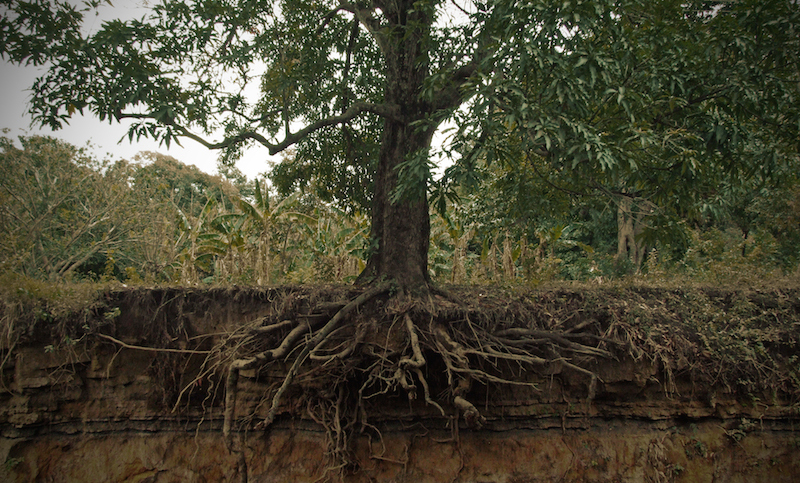
\includegraphics[height=7.2cm]{tree-scary.jpg}
\end{center}
\end{frame}

\begin{frame}[fragile]{Key example}
\texttt{List[Int]}
\end{frame}

\begin{frame}[fragile]{Key example}
\begin{semiverbatim}
\small
scala> t"List[Int]".show[Raw]
res1: String =
Type.Apply(Type.Name("List"), List(Type.Name("Int")))

\only<2>{scala> t"\text{\color{blue}{List}}[\text{\color{red}{Int}}]".show[Semantics]}
\only<2>{res2: String =}
\only<2>{Type.Apply(\text{\color{blue}{Type.Name("List")[1]}}, List(\text{\color{red}{Type.Name("Int")[2]}}))}
\only<2>{[1] Type.Singleton(Term.Name("package")[4])::scala.package#List}
\only<2>{[2] Type.Singleton(Term.Name("scala")[3])::scala#Int}
\only<2>{...}
\end{semiverbatim}
\end{frame}

\begin{frame}[fragile]{Name resolution}
\begin{semiverbatim}
scala> implicit val c = Scalahost.mkStandaloneContext()
c: scala.meta.macros.Context = ...

scala> q"scala.collection.immutable.List".defn
res3: scala.meta.Member.Term = object List extends
SeqFactory[List] with Serializable \{ ... \}

scala> res3.name
res4: scala.meta.Term.Name = List
\end{semiverbatim}
\end{frame}

\begin{frame}[fragile]{Other semantic APIs}
\begin{semiverbatim}
scala> q"scala.collection.immutable.List".defs("apply")
res5: scala.meta.Member.Term =
override def apply[A](xs: A*): List[A] = ???

scala> q"scala.collection.immutable.List".parents
res6: Seq[scala.meta.Member.Term] =
List(abstract class SeqFactory...)
\end{semiverbatim}
\end{frame}

\begin{frame}{Derived technologies}
First-class names enable:
\begin{itemize}
\item Unification of trees, types and symbols
\item Referential transparency and hygiene (under development!)
\item Simpler mental model of metaprogramming
\end{itemize}
\end{frame}

\sectionframe{Wrapping up}

\begin{frame}{Summary}
\vskip45pt
\begin{itemize}
\item scala.meta is a one-stop solution to frontend metaprogramming
\item Our key innovations include first-class support for tokens and names
\item This gives rise to a powerful, yet simple model of Scala programs
\item We are working hard to provide an alpha release soon
\end{itemize}
\vskip25pt
\visible<2>{Upcoming presentations:\\}
\visible<2>{Live demo at a Scala Bay meetup in Mountain View (19 March)\\}
\visible<2>{Hands-on workshop at flatMap in Oslo (27-28 April)\\}
\visible<2>{Next status update at ScalaDays in Amsterdam (8-10 June)}
\end{frame}

\end{document}
